% Welcome to the LaTeX code for this lab report template.
% Comments start with '%'

% This is were we specify the overall class of document you are creating. You don't need to change this.
\documentclass[12pt, letterpaper]{article}

% These commands are like including header files
\usepackage[utf8]{inputenc}
\usepackage{hyperref}
\usepackage{epsfig, url}
\usepackage{epstopdf}
\usepackage{graphicx}
\usepackage{datetime}
\usepackage{multirow}

%\usepackage{wrapfig}
%\usepackage{amsmath}
\usepackage{amssymb}
\usepackage{geometry} 
\geometry{a4paper}              

\usepackage{titling}

%\documentclass{article}
\usepackage{xcolor}
\usepackage{listings}

\definecolor{mGreen}{rgb}{0,0.6,0}
\definecolor{mGray}{rgb}{0.5,0.5,0.5}
\definecolor{mPurple}{rgb}{0.58,0,0.82}
\definecolor{backgroundColour}{rgb}{0.95,0.95,0.92}

\lstdefinestyle{CStyle}{
    backgroundcolor=\color{backgroundColour},   
    commentstyle=\color{mGreen},
    keywordstyle=\color{magenta},
    numberstyle=\tiny\color{mGray},
    stringstyle=\color{mPurple},
    basicstyle=\footnotesize,
    breakatwhitespace=false,         
    breaklines=true,                 
    captionpos=b,                    
    keepspaces=true,                 
    numbers=left,                    
    numbersep=5pt,                  
    showspaces=false,                
    showstringspaces=false,
    showtabs=false,                  
    tabsize=2,
    language=C
}

\usepackage{indentfirst}
\setlength{\evensidemargin}{0in}
\setlength{\oddsidemargin}{0in}
\setlength{\textwidth}{6.5in}
\setlength{\textheight}{9.0in}
\setlength{\topmargin}{0in}
\setlength{\headheight}{0in}
\setlength{\headsep}{0in}
\setlength{\itemsep}{-\parsep}



% This command starts the document
\begin{document}

% This command says to include all the LaTeX code from titlepage.tex, which includes the Title Page.
%Go edit the titlepage.txt code first. Then come back here.
% Change NUM below with the lab number:
\title{\large ECEN 260 - Final Project\\[0.5cm]
        % Change "Lab Title Here" below with the lab title:
        \bf\Large Handheld Snake Game}

% Change "Your Name Here" to be your name.
\author{\large Jacob Lamb}

% Change "Month Day, 2024" to be the current date:
\date{Decemebr 16, 2024}
\makeatletter
    \begin{titlepage}
        \begin{center}
        \vfill 
\includegraphics[scale=1]{images/banner}\\[2cm]
        \vbox{}\vspace{1cm}
            {\@title }\\[3cm] 
            {\@author}\\[10cm]

            % Change XXXX to be the name of your instructor 
            {Instructor: Brother Allred}\\
            
            {\@date}
        \end{center}
    \end{titlepage}
\makeatother

% After making changes, click the "Recompile" button to regenerate your pdf from the updated code.
% Now, go back to main.tex

\newpage

% This command will automatically generate a table of contents, based on what is in the rest of the document.
% You don't need to change this code.
\tableofcontents
\newpage

% These commands will find all tables and figures in the document and create a reference to them.
% You don't need to change this code.
\listoftables
\listoffigures
\newpage

% This command says to include all the LaTeX code from overview.tex, which includes the Lab Overview Section.
% Go edit the overview.tex code next. Then come back here.
% This command makes a section called "Lab Overviewe"
\section{Project Overview}
\label{sec:objectives} % This tags the section so we can reference it.

This project demonstrates the development of a classic Snake Game implemented on a Nucleo board, utilizing embedded systems concepts. The game operates within a constrained play area, where the snake's movement is restricted by borders, and the game ends upon collision with the borders or upon collision with the snake body.

A key focus of the project was the integration of hardware and software components, including the use of SPI displays, timers, and interrupts to create a responsive and engaging user experience. These components were managed in real-time to ensure smooth gameplay mechanics, such as boundary collision detection and player input handling. This project was developed as part of a course on microprocessors and I/O devices, highlighting practical applications of the concepts covered in the class. 

% This command makes another subsection within the current section
\subsection{Objectives}

\begin{itemize}
    \item Design and implement a game with responsive controls and gameplay mechanics.
    \item Use the Nucleo board and an SPI display to create a visually engaging and interactive user interface.
    \item Demonstrate the use of timers and interrupts to manage real-time game logic and inputs efficiently.
  
\end{itemize}

\newpage

% This command says to include all the LaTeX code from specifications.tex, which includes the Specifications Section.
% Go edit the specifications.tex code next. Then come back here.
\section{Specifications}
\label{sec:specifications}


    This project utilizes a Nucleo board connected to an SPI display and four push buttons, with each button configured as an interrupt. For detailed wiring instructions, refer to the schematics in Section \ref{sec:schematic}. The program initializes by displaying the border of the play area before the game begins. The game is started by pressing any of the four buttons. Once the game ends, the reset button on the Nucleo board allows the user to restart the game.

    The game begins with the snake spawning at the center of the screen, starting with an initial length of three. A "food" spot is also randomly generated on the screen. The user controls the snake's movement using the four buttons, with each button corresponding to a direction: up, down, left, or right. Every time the snake consumes a food spot, its length increases. The game ends if the snake collides with the border or its own body, at which point a "Game Over" message is displayed. If the snake reaches the maximum possible length of 48 (the capacity of the play area), a "Winner" message is displayed.
     
     

\subsection{Parts List}

\begin{itemize}
    \item Nucleo-L476RG board and USB cable
    \item PCD8544 GLCD screen
    \item 4 push buttons
    \item several jumper wires
\end{itemize}


\newpage

% This command says to include all the LaTeX code from schematics.tex, which includes the Schematics Section.
% Upload your schematics image file into the "images" folder to the left.
% Then go edit the schematics.tex file to reference your image.
\section{Schematics}
\label{sec:schematic}


\begin{figure}[h!]
    \centering
    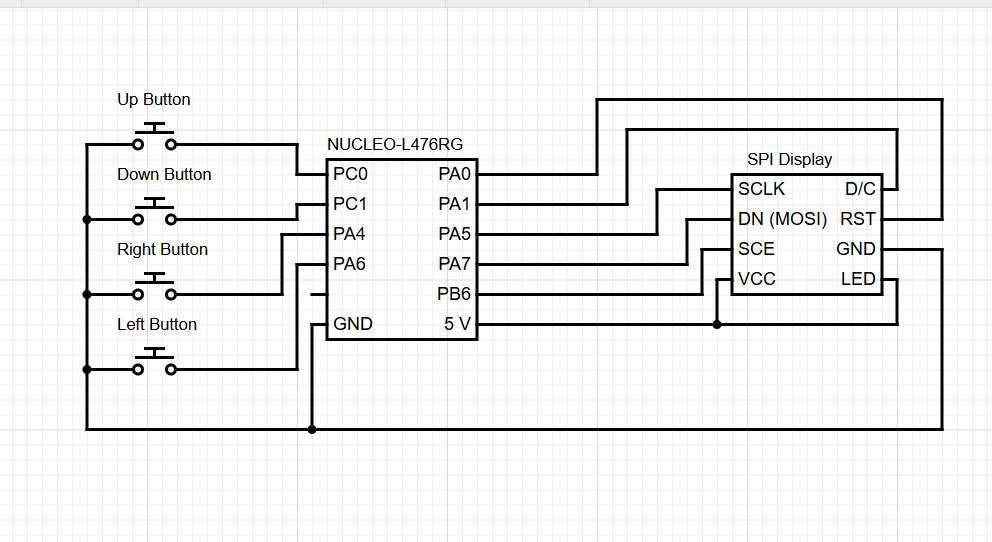
\includegraphics[scale= 0.5]{images/schematic.png}
    \caption{Schematic diagram for the Lab.}
    \label{fig:schematic}
\end{figure}

\newpage

% This command says to include all the LaTeX code from test.tex, which includes the Test Plan and Test Results Section.
\section{Test Plan and Test Results}
\label{sec:test}

The test procedure for the snake game ensures that all key features of the game function as expected. The tests begin with powering on the Nucleo board and verifying that the play area border is displayed. Once the game starts, each of the four buttons—up, down, left, and right—is tested to confirm that the snake moves in the correct direction when pressed. The game also tests the snake’s ability to grow when consuming food and checks if the game properly ends when the snake collides with the border or its own body. Finally, the test ensures that the game correctly displays a "Winner" message when the snake reaches its maximum length and that the reset button functions to restart the game. This procedure verifies the core gameplay mechanics and ensures the expected results for each action.

\subsection{Test Plan Procedure and Results}
\begin{table}[h!]
\centering
\renewcommand{\arraystretch}{1.2}
\begin{tabular}{|p{5cm}|p{6cm}|p{4cm}|}
\hline
\textbf{Step} & \textbf{Expected Result} & \textbf{Actual Result} \\
\hline
Power on the Nucleo board. & Play area border is displayed; game is idle. & Play area border displayed; game idle. \\ 
\hline
Press any button to start the game. & Snake spawns at center with initial length of 3; food appears. & Snake spawned at center with initial length of 3; food appeared. \\ 
\hline
Press the "Up" button. & Snake moves upward on the screen. & Snake moved upward on the screen. \\ 
\hline
Press the "Down" button. & Snake changes direction downward. & Snake changed direction downward. \\ 
\hline
Press the "Left" button. & Snake changes direction left. & Snake changed direction left. \\ 
\hline
Press the "Right" button. & Snake changes direction right. & Snake changed direction right. \\ 
\hline
Move the snake to a food spot. & Snake grows by one unit; new food appears. & Snake grew by one unit; new food appeared. \\ 
\hline
Collide the snake with the border. & "Game Over" message appears. & "Game Over" displayed. \\ 
\hline
Collide the snake with its own body. & "Game Over" message appears. & "Game Over" displayed. \\ 
\hline
Reach snake length of 48. & Winner message appears. & Winner message displayed. \\ 
\hline
Press the reset button. & Game resets; play area border displayed again. & Game reset; play area border displayed again. \\ 
\hline
\end{tabular}
\caption{Snake Game Test Procedures}
\label{tab:test_procedures}
\end{table}





\newpage  

% This command says to include all the LaTeX code from code.tex, which includes the Code Section.
% This command makes a section called "Code"
\section{Code}
\label{sec:code}

Below are selected portions of the code used to create the Snake Game. These snippets highlight the most critical components that drive the core functionality of the game. The most important parts of the code are found in the callback functions for the interrupts of the buttons being pushed and the interrupt of the timer for the game being triggered. 
\ref{subsec:main_c} having the code for main.c.

% This command makes a subsection
\subsection{Code for main.c}
\label{subsec:main_c}

% Put code between "lstlisting" commands using the CStyle tag, like this:
\begin{lstlisting}[style=CStyle]

uint32_t lastButtonPressTime = 0;   // Last valid press time (in ms)

bool gameStart = false; 			// player needs to press any button to start the game, this boolean will become true
bool gameOver = false;				// this variable becomes true when the user looses the game
bool gameWin = false;				// this variable becomes true if the user wins the game (snake length = 60)

char direction = 'R';				// The initial direction of the snake is always right

typedef struct {
    int x;
    int y;
} Point;

Point snake[59]; 				// Snake body
int snakeLength = 3;           	// Initial length of the snake
Point food;                   	// Position of the food


main{
  //Initial snake position
  snake[0] = (Point){6, 2}; // Initial head position
  snake[1] = (Point){5, 2}; // Initial body
  snake[2] = (Point){4, 2}; // Initial body
  placeFood();

  GLCD_init();  // initialize the screen
  GLCD_clear(); // clear the screen
  // Draw borders
  for (int x = 0; x < maxX; x++) {
      GLCD_setCursor(x * 6, 0);
      GLCD_putchar(23); // Top border
      GLCD_setCursor(x * 6, NUM_BANKS - 1);
      GLCD_putchar(23); // Bottom border
  }
  for (int y = 0; y < maxY + 1; y++) {
      GLCD_setCursor(0, y );
      GLCD_putchar(23); // Left border
      GLCD_setCursor(GLCD_WIDTH - 6, y );
      GLCD_putchar(23); // Right border
  }

  HAL_TIM_Base_Start_IT(&htim16); // Start Timer 16
}

//Interrupt function for game timer
void HAL_TIM_PeriodElapsedCallback(TIM_HandleTypeDef *htim) {
	// htim16 is the timer set for the game
	// the game will start when a button is pushed

    if (htim == &htim16 && gameStart && !gameOver && !gameWin) {
    	//These three functions control the game mechanics
        moveSnake();
        checkCollision();
        drawGame();

	}
    //The game over
    if (gameOver)
    {
    	GLCD_setCursor(12,2);
    	//GAME OVER
    	// 28 1 29 5 0 11 30 5 31
    	GLCD_putchar(28);	//G
    	GLCD_putchar(1);	//A
    	GLCD_putchar(29);	//M
    	GLCD_putchar(5);	//E
    	GLCD_putchar(0);	//space
    	GLCD_putchar(11);	//O
    	GLCD_putchar(30);	//V
    	GLCD_putchar(5);	//E
    	GLCD_putchar(31);	//R
    }

    if (gameWin){
    	GLCD_setCursor(12,2);
    	GLCD_putchar(8);	//W

    }
}

//Interupt function when a button is pushed
void HAL_GPIO_EXTI_Callback(uint16_t GPIO_Pin) {
	
	//To debounce Buttons
	uint32_t currentTime = HAL_GetTick();
	uint32_t timeSinceLastButton = currentTime - lastButtonPressTime;
		
	//The first button push will start the game. The game will start with the snake going right no matter what button is pushed
	if (!gameStart){
		gameStart = true;

	} else{
		
	//This if statement is for button denouncing
	if (timeSinceLastButton > 100){
		
		//The direction of the snake will change depending on which button was pushed
		if (GPIO_Pin == UpB_Pin){
			direction = 'U';
		}
		if (GPIO_Pin == DownB_Pin){
			direction = 'D';
			}
		if (GPIO_Pin == LeftB_Pin){
			direction = 'L';
			}
		if (GPIO_Pin == RightB_Pin){
			direction = 'R';
			}
		}
	}
	lastButtonPressTime = HAL_GetTick();
}

void moveSnake() {
    // Check if the snake eats the food
    if (snake[0].x == food.x && snake[0].y == food.y) {
        snakeLength++;
        if (snakeLength == 48) {//48 is the maximum spaces on the SPI board, therefore the game is won when the length = 60
        	gameWin = true;
        	gameStart = false;

        }else{
        placeFood();		//If the snake gets food and the game has not been won, new food must be placed.
        }
    }

	// Move the snake's body
    for (int i = snakeLength - 1; i > 0; i--) {
        snake[i] = snake[i - 1];
    }

    // Move the head
    if (direction == 'U') snake[0].y--;
    if (direction == 'D') snake[0].y++;
    if (direction == 'L') snake[0].x--;
    if (direction == 'R') snake[0].x++;


}

void checkCollision() {
    // Check wall collision
    if (snake[0].x < 1 || snake[0].x >= maxX || snake[0].y < 1 || snake[0].y >= maxY) {
        gameOver = true;
        return;
    }

    // Check self-collision
    for (int i = 1; i < snakeLength; i++) {
        if (snake[0].x == snake[i].x && snake[0].y == snake[i].y) {
            gameOver = true;
            return;
        }
    }
}

void drawGame() {
    GLCD_clear();
    // Draw borders
    for (int x = 0; x < maxX; x++) {
        GLCD_setCursor(x * 6, 0);
        GLCD_putchar(23); // Top border
        GLCD_setCursor(x * 6, NUM_BANKS - 1);
        GLCD_putchar(23); // Bottom border
    }
    for (int y = 0; y < maxY + 1; y++) {
        GLCD_setCursor(0, y );
        GLCD_putchar(23); // Left border
        GLCD_setCursor(GLCD_WIDTH - 6, y );
        GLCD_putchar(23); // Right border
    }

    // Draw the snake
    for (int i = 0; i < snakeLength; i++) {
        GLCD_setCursor(snake[i].x * 6, snake[i].y);
        GLCD_putchar(14); // Snake body
    }

    // Draw the food
    GLCD_setCursor(food.x * 6, food.y);
    GLCD_putchar(27); // Food
}

void placeFood() {
	int isOccupied = 1;
	do {
        // Generate random coordinates for food
        food.x = 1 + rand() % (maxX - 1);  // This ensures x is between 1 and maxX-1
        food.y = 1 + rand() % (maxY - 1);  // This ensures y is between 1 and maxY-1

        // Check if the food position is occupied by the snake
        isOccupied = 0;
        for (int i = 0; i < snakeLength; i++) {
            if (snake[i].x == food.x && snake[i].y == food.y) {
                isOccupied = 1; // Food position is occupied by the snake
                break; // No need to check further if the position is already taken
            }
        }

    } while (isOccupied); // Repeat if the food is in the snake's body
}
void GLCD_putchar(int font_table_row){
	int i;
	for (i=0; i<6; i++){
		GLCD_data_write(font_table[font_table_row][i]);
	}
}

void SPI_write(unsigned char data){
	// Chip Enable (low is asserted)
	HAL_GPIO_WritePin(CE_PORT, CE_PIN, GPIO_PIN_RESET);


	// Send data over SPI1
	HAL_SPI_Transmit(&hspi1, (uint8_t*) &data, 1, HAL_MAX_DELAY);

	// Chip Disable
	HAL_GPIO_WritePin(CE_PORT, CE_PIN, GPIO_PIN_SET);
}

void GLCD_data_write(unsigned char data){
	//Switch to "data" mode (D/C pin high)
	HAL_GPIO_WritePin(DC_PORT, DC_PIN, GPIO_PIN_SET);

	// Send data over SPI
	SPI_write(data);
}

void GLCD_command_write(unsigned char data){
	//Switch to "command" mode (D/C pin low)
	HAL_GPIO_WritePin(DC_PORT, DC_PIN, GPIO_PIN_RESET);

	// Send data over SPI
	SPI_write(data);
}

void GLCD_init(void){

	// Keep CE high when not transmitting
	HAL_GPIO_WritePin(CE_PORT, CE_PIN, GPIO_PIN_SET);

	//Reset the screen (low pulse - down and up)
	HAL_GPIO_WritePin(RESET_PORT, RESET_PIN, GPIO_PIN_RESET);
	HAL_GPIO_WritePin(RESET_PORT, RESET_PIN, GPIO_PIN_SET);

	//Configure the screen according to the datasheet
	GLCD_command_write(0x21); //enter extended command mode
	GLCD_command_write(0xC4); //Set LCD Vop for contrast (this may be adjusted)
	GLCD_command_write(0x04); //set temp coefficient
	GLCD_command_write(0x10); //set LCD bias mode (this may be adjusted)
	GLCD_command_write(0x20); //return to normal command mode
	GLCD_command_write(0x0C); //set display mode normal
}

void GLCD_setCursor(unsigned char x, unsigned char y){
	GLCD_command_write(0x80 | x);	//column
	GLCD_command_write(0x40 | y);	//bank
}

void GLCD_clear(void){
	int i;
	for(i = 0; i < (GLCD_WIDTH * NUM_BANKS); i++){
		GLCD_data_write(0x00); //write zeros
	}
	GLCD_setCursor(0,0);	//return cursor to top left
}


\end{lstlisting}

\newpage

% This command says to include all the LaTeX code from discussion.tex, which includes the Discussion and Conclusion Section.
% This command makes a section called "Code"
\section{Conclusion}

% Paragraph 1
The Snake Game project provided an excellent opportunity to exercise and expand my knowledge of embedded systems. Through this project, I effectively integrated three major course concepts: SPI displays, timers, and interrupts, demonstrating a clear understanding of their functions and interplay. The use of an SPI display required precise pixel control to render game elements, while timers regulated the snake’s movement and game pacing, ensuring smooth and consistent gameplay. Interrupts were essential for handling real-time input from the push buttons, allowing for a responsive and user-friendly interface.

This project highlighted the practical applications of embedded systems, emphasizing how these components work together to create an interactive and efficient system. The challenges of coordinating these elements provided valuable hands-on experience that deepened my understanding of hardware-software integration.

Beyond its technical achievements, the project reinforced the importance of simplicity and functionality in design. By focusing on user-friendly controls and efficient operation, I created a portable and engaging game that demonstrates the capabilities of embedded systems. This project served as a meaningful step toward solving real-world engineering problems and showcased my ability to apply technical concepts in a creative and impactful way.
 

\newpage

% These commands generate your references from the __ref.bib file using the IEEE standard.
\bibliographystyle{ieeetr}
\bibliography{__ref}

% This command ends the document
\end{document}
